%!TEX root = ../thesis.tex
%*******************************************************************************
%****************************** Second Chapter *********************************
%*******************************************************************************

\chapter{STUDI PENDAHULUAN}

\ifpdf
    \graphicspath{{Chapter2/Figs/Raster/}{Chapter2/Figs/PDF/}{Chapter2/Figs/}}
\else
    \graphicspath{{Chapter2/Figs/Vector/}{Chapter2/Figs/}}
\fi

\section{Macam Macam Operasi Pasca Bencana}
Lorem ipsum dolor sit amet, consectetur adipiscing elit. Nullam ante quam, varius id tincidunt in, aliquet gravida felis. Praesent vehicula risus at pulvinar mattis. Duis feugiat diam ut massa euismod mollis. Maecenas tempus nisl diam, et sodales massa pharetra ut. Duis id ipsum ut dolor tincidunt euismod vitae sed odio. Duis tincidunt lorem ac leo mattis varius. Sed mollis metus nec tempor congue. Ut imperdiet dui ut ante mollis auctor. Suspendisse sit amet scelerisque sapien, in cursus nisl. Etiam egestas tellus mi, non fringilla justo ultricies at. Praesent eget ipsum porta, fermentum lorem sit amet, suscipit ligula. Nulla porttitor finibus neque nec sodales. Orci varius natoque penatibus et magnis dis parturient montes, nascetur ridiculus mus. Maecenas auctor quam ut justo accumsan, consequat eleifend massa imperdiet. Ut dictum eleifend justo, vitae pellentesque eros porta id.

Aenean dapibus dolor ac fermentum ornare. Sed feugiat augue non aliquet hendrerit. Nulla quis neque ultrices, convallis nisl at, posuere justo. Duis ultrices neque et urna ornare fringilla. Mauris eget porttitor nulla. Etiam porttitor nisl est, ornare posuere turpis fringilla at. Quisque varius augue orci, eu molestie erat luctus sed. Fusce quis venenatis nisi. Pellentesque interdum nibh a nibh elementum mollis. Aliquam at scelerisque nibh.

Nullam egestas diam mi, id lacinia sapien accumsan in. Nulla ornare, ex non pulvinar feugiat, est magna luctus elit, id rutrum orci libero at mi. Nullam elementum condimentum feugiat. Curabitur porta vel magna non vestibulum. Maecenas placerat ipsum at interdum tincidunt. Morbi aliquam fringilla justo sed tristique. Duis egestas erat tristique, ornare sapien eu, hendrerit magna. Nunc nec tincidunt nisl. Integer vulputate quam diam, a pellentesque ante blandit vel. Orci varius natoque penatibus et magnis dis parturient montes, nascetur ridiculus mus. Ut elementum pharetra lacus, non cursus nisl auctor sit amet. Nunc feugiat sagittis lectus, in rhoncus ante vestibulum ut. Vivamus pulvinar eget nisl sed feugiat. Nam eget dolor imperdiet, interdum dolor imperdiet, rutrum lorem.

Sed pharetra vel nulla ac varius. Curabitur consectetur felis sit amet enim dapibus, eget semper neque viverra. Mauris vitae risus ut urna mollis semper in ac arcu. Donec vitae pharetra dui. Nam posuere egestas finibus. Sed eleifend varius sapien ut tristique. Curabitur sodales at erat at volutpat. Suspendisse non nunc eu magna sollicitudin sagittis. Nunc ullamcorper, lectus posuere vulputate tincidunt, lectus mauris eleifend enim, ac sodales tortor diam sed tellus. Aliquam at lacus ante. Cras mollis purus at euismod aliquet. Suspendisse potenti. Quisque venenatis non urna eget tristique. Nam vestibulum eu est vitae dignissim. Nulla sollicitudin convallis nisi, in luctus massa rutrum eu. Nulla commodo velit ac pulvinar lacinia.

Donec enim nunc, aliquet vel blandit in, sagittis porta eros. Vestibulum non vulputate tortor, ac bibendum nunc. Praesent orci quam, tincidunt ac fermentum at, sodales sit amet justo. Interdum et malesuada fames ac ante ipsum primis in faucibus. Vivamus dictum risus ut euismod sollicitudin. Donec efficitur, massa sed vestibulum rutrum, massa quam elementum lacus, sit amet commodo libero neque non dui. Vestibulum velit sem, rutrum sed blandit vitae, tincidunt feugiat enim. Nam vestibulum rhoncus lorem. Ut varius erat sem, eu finibus lorem tristique ac. Donec non fermentum magna. Pellentesque habitant morbi tristique senectus et netus et malesuada fames ac turpis egestas.

\section{Robot untuk Bencana}
\subsection{Pengertian Robot untuk Bencana}
\textit{Rescue robot} pertama kali digunakan pada program Tactical Mobile Robots oleh Defense Advanced Research Projects Agency (DARPA) bekerja sama dengan Center for Robot-Assisted Search and Rescue (CRASAR) untuk misi bencana World Trade Center di New York tahun 2001. Penelitian akademik tentang rescue robotics dimulai tahun 1995 oleh dua kelompok riset yaitu grup Prof. Satoshi Takokoro dari Kobe University, Jepang dan kelompok Robin R. Murphy dari Colorado School of Mines, Amerika Serikat. 

\textit{Rescue robot} termasuk kategori mobile robot yang secara umum berukuran kecil dan portabel untuk dibawa, digunakan dan dioperasikan sesuai kebutuhan oleh sebuah grup yang membutuhkan informasi darinya, dalam hal ini tim SAR. \textit{Rescue robot} berbeda dengan mobile robot untuk industri yang biasanya melakukan tugas yang sama berulang-ulang. \textit{Rescue robot} biasa ditempatkan pada  lingkungan yang tidak terduga sehingga diharuskan mampu untuk mengetahui keadaan sekitar \citet{murphy2016disaster}.

\textit{Mobile robot} sering disebut dengan unmanned system (sistem tak berawak) untuk membedakan dengan robot yang biasa digunakan dalam industri. Robot tersebut terbagi atas tiga modalitas berdasarkan di mana mereka beroperasi, yaitu
\begin{enumerate}
 \item Jika beroperasi di tanah, robot disebut unmanned ground vehicles (UGV).
 \item Jika beroperasi di air, mereka termasuk dalam kategori umum unmanned marine vehicles (UMV) yang nantinya dapat dibagi lagi kedalam unmanned surface vehicles (USV) untuk di atas permukaan air dan unmanned underwater vehicles (UUV) untuk di bawah permukaan laut.
 \item Jika beroperasi di udara, robot biasa disebut dengan berbagai nama yaitu unmanned aerial vehicles (UAVs), unmanned aerial systems (UASs), remotely piloted aircraft (RPA), or remotely piloted vehicles (RPVs). UAV sendiri terdiri dari dua kategori yaitu fixed wing (memiliki bentuk seperti pesawat) dan VTOL (vertical takeoff and landing, memiliki bentuk seperti helikopter).
\end{enumerate}

\begin{table}[ht]
\centering
\caption{Pengembangan Disaster Robot dari 2001 hingga 2013 Berdasarkan Jenis dan Banyaknya}
\captionsetup{font={footnotesize}}
\caption*{Sumber: \citet{murphy2016disaster}, halaman 35}
\label{table:pengembangan_robot}
\resizebox{\textwidth}{!}{%
\begin{tabular}[\textwidth] { c c c c c | c c c c c}
\hline 
&  &  \multicolumn{3}{c}{Modality} &  & & \multicolumn{2}{c}{Modality} \\
Disaster & Deployement & Ground & Aerial & Marine & Disaster  & Deployement & Ground & Aerial & Marine \\
Year & Event &  &  &  & Year & Event &  &  &  \\
\hline
2001 & World Trade Center (USA) & 4 & & & 2001 & Hurricane Ike (USA)& & &1 \\
2001 & Jim Walter No.5 Mine (USA) & 1 & & & 2001 &Historical Archive of cologne & 2 & & \\
& & & & & & building collapse (Germany) & & & \\
2002 & Barrick Gold Dee Mine (USA) & 1 & & & 2002 & L'Aquila earthquake (Italy) & &1 & \\
2004 & Brown's Fork Mine (USA) & 1 & & & 2004 &Haiti earthquake & & 1& 1\\
2004 & Niigata Chuetsu earthquake (Japan) & 1 & & & 2004 & Wangjialing Coal Mine (China)& 1& & \\
2004 & Hurricane Charley (USA) & 1 & & & 2004 & Upper Big Branch Mine (USA)&1 & & \\
2004 & Excel No.3 Mine (USA) & 1 & & & 2004 & Deepwater Horizon (USA)& & &16 \\
2005 & DR No. 1 Mine (USA) & 1 & & & 2005 &Prospect Towers (USA) &2 & & \\
2005 & McClane Canyone Mine (USA) & 1 & & & 2005 & Missing Balloonist (Italy)& & &1 \\
2005 & La Conchita medslides (USA) & 1 & & & 2005 & Pike River Mine (New Zealand)& 2& & \\ 
2005 & Hurricane Katrina (USA) & 1 & 3 & & 2005 & Christchurch earthquake (NZ)&1 &1 & \\
2005 & Hurricane Wilma (USA) & & 1 & 1 & 2005 &Tohoku earthquake (Japan) &3 &1 & \\
2006 & Sago Mine (USA) & 1 & & & 2006 & Tohoku Tsunami (Japan)& & &9 \\
2007 & Midas Gold Mine (USA) & 2 & & & 2007 & Fukushima Daiichi Nuclear & 7&2 & \\
 &  &  & & & & Emergency (Japan) & & & \\
2007 & Crandall Canyon Mine (USA) & 1 & & & 2007 & Naval base explosion (Cyprus) & &2 & \\
2007 & I-35 Minnesota Bridge Collapse (USA) & & & 2 & 2007 & Great Thailand Flood (Thailand)& &2 & \\
2007 & Berkmall Plaza II Collapse & 2 & 1 & & 2007 &Finale Emilia earthquake (Italy) &2 &2 & \\
\hline 
\end{tabular} }
\end{table}

Terlihat dari Tabel ~\ref{table:pengembangan_robot}, model \textit{Rescue robot} yang paling banyak digunakan dalam misi yang sesungguhnya adalah UGV. Namun sejak tahun 2011, UAV mulai banyak digunakan. Hal tersebut dikarenakan kemampuan jelajah UAV yang lebih bebas dan cepat dibandingkan dengan UGV sehingga mampu mencari pada area yang lebih luas.

Pada sub bab selanjutnya akan dijelaskan tentang penelitian pencarian korban bencana alam baik menggunakan UGV maupun UAV. Perbedaan keduanya adalah sudut pandang tanah dan sudut pandang udara.

\subsection{Penelitian Robot untuk Bencana Sebelumnya}
\begin{figure}[ht]
 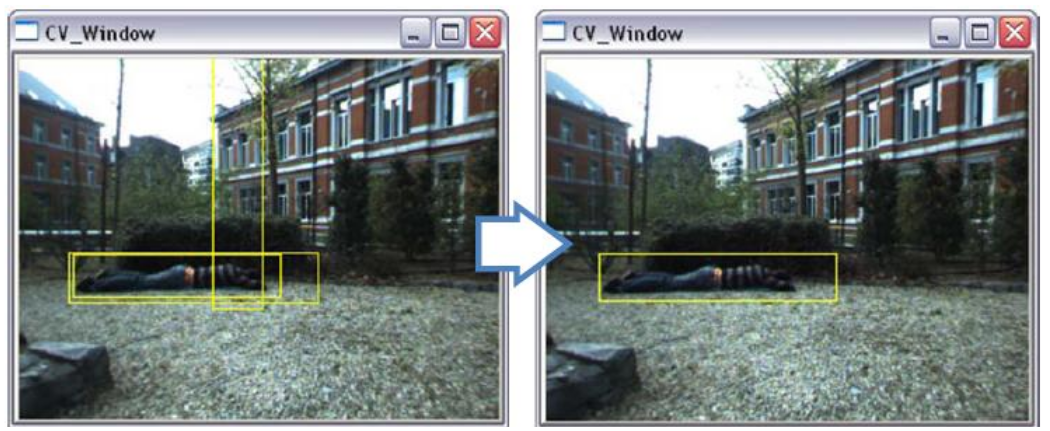
\includegraphics[width=\textwidth]{Decuber}
 \caption{Deteksi Korban pada tanah lapang oleh \cite{de2009human}}
  \captionsetup{font={footnotesize}}  
  \caption*{Sumber: \citet{de2009human}, halaman 8}
 \label{fig:deteksidecuber}   
\end{figure}

Salah satu contoh deteksi pada pandangan tanah yang dibahas adalah milik \citet{de2009human}, dimana proses pengenalan korban menggunakan kamera. Sistem mendeteksi dengan Cascade Haar-features Classifier lalu mengembangkan teknik Viola-Jones Face and Upper Body Detection untuk menentukan korban. Dataset yang digunakan merupakan gambar manusia telungkup pada daerah lapang. Deteksi mencapai akurasi 100\% pada dataset seperti Gambar~\ref{fig:deteksidecuber}, namun turun hingga rata rata 65\% ketika berada pada posisi yang berbeda.

Selain itu, robot iSRo-G2 merupakan UGV yang dikembangkan oleh \citet{Irawan2011isro} dimana robot menggunakan sensor kamera dan sensor PIR. Penggunaan sensor kamera masih belum dapat optimal dimana tidak dapat membedakan warna kulit dengan warna coklat. Program yang digunakan untuk deteksi pada kamera masih harus dikembangkan selain menggunakan metode Ant Colony Optimization.

Pencarian korban bencana alam dengan UGV menggunakan sudut pandang dari tanah (ground) sehingga jangkauan penglihatan tidak terlalu besar. \citet{blondel2014human}, menjelaskan tentang perbedaan untuk mendeteksi manusia pada sudut pandang tanah dengan sudut pandang UAV. Percobaan menekankan perhitungan sudut pengambilan gambar pada deteksi manusia menggunakan UAV. Percobaan tersebut mengoptimalisasi Histograms of Oriented Gradients (HOG) yang diuji coba pada dataset INRIA dan GMVRT-V1 dimana merupakan dataset manusia pada kondisi normal.

UAV robot salah satunya di kembangkan oleh \citet{andriluka2010vision}. Penelitian tersebut menguji coba berbagai macam metode seperti Histograms of Oriented Gradients (HOG), Poselets-based Detector (PDB), Discriminatively trained Part based Models (DPM), Pictorial Structures (PS), dan DPM + PS. Hasil terbaik didapatkan dengan metode DPM+PD. Seperti terlihat pada Gambar~\ref{fig:andriluka}. pengujian dan dataset yang digunakan dilakukan pada lokasi dalam ruangan dan tidak merepresentasikan kondisi bencana alam yang sesungguhnya.

\begin{figure}[ht]
 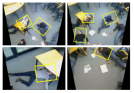
\includegraphics[width=\textwidth]{andriluka}
 \caption{Hasil Pengujian Deteksi Korban oleh \cite{andriluka2010vision}}
   \captionsetup{font={footnotesize}}
  \caption*{Sumber: \citet{andriluka2010vision}, halaman 1}
 \label{fig:andriluka}   
\end{figure}

Penelitian menggunakan UAV juga dilakukan oleh \citet{doherty2007uav}. Pada penelitian ini digunakan gabungan dari dua jenis kamera yaitu kamera thermal dan kamera biasa seperti Gambar~\ref{fig:doherty}. Kamera termal menangkap panas dari treshold rata rata panas manusia yang telah ditentukan untuk proses deteksi awal. Selanjutnya, gambar termal akan dicocokan dengan gambar normal menggunakan Cascade Haar-like features. Dengan adanya dua buah sensor tersebut akan meningkatkan akurasi deteksi namun  penambahan berat sensor pada UAV dan proses deteksi yang lebih kompleks.

\begin{figure}[ht]
 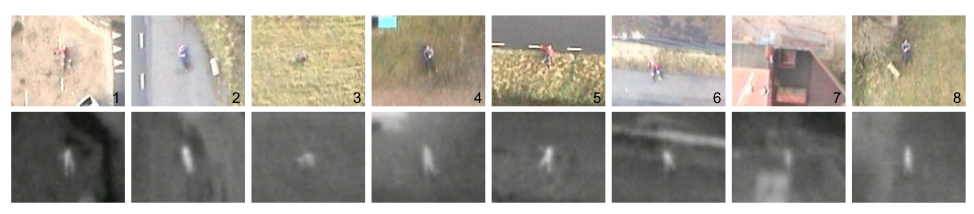
\includegraphics[width=\textwidth]{doherty}
 \caption{Penggabungan Kamera dan Termal oleh \cite{doherty2007uav}}
   \captionsetup{font={footnotesize}}
  \caption*{Sumber: \citet{doherty2007uav}, halaman 9}
 \label{fig:doherty}   
\end{figure}

\citet{kuntze2014situation}, mengembangkan rescue robot bernama SENEKA yang terdiri dari ground station, human operators, UAV, UGV dan sensor system. Dengan berbagai macam sensor dan robot yang diletakan pada area bencana membuat akurasi deteksi korban menjadi lebih tinggi. Namun dalam penelitian tersebut masih dibutuhkan human operator untuk memberikan perintah semi-autonomous kepada masing masing robot dan deteksi secara manual. Cara kerja dari sistem ini diilustrasikan pada Gambar~\ref{fig:kuntze}.

\begin{figure}[ht]
 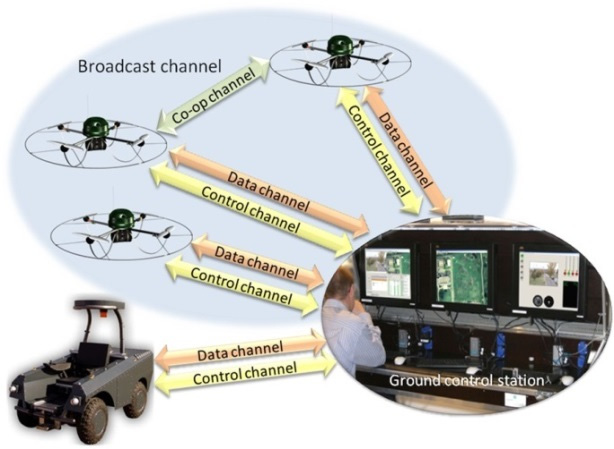
\includegraphics[width=\textwidth/2]{kuntze}
 \caption{Hasil Pengujian Deteksi Korban oleh \cite{kuntze2014situation}}
   \captionsetup{font={footnotesize}}
  \caption*{Sumber: \citet{kuntze2014situation}, halaman 3}
 \label{fig:kuntze}   
\end{figure}

\section{Deep Learning}
\subsection{Pengertian dan Deep Learning}
Deep learning termasuk dalam kelas Machine Learning, dimana komputer akan memiliki kemampuan untuk belajar tanpa diprogram secara eksplisit. Machine Learning merupakan salah satu teknik Kecerdasan Buatan (Artificial Intelligence) yang memungkinkan mesin meniru kecerdasan manusia, dalam hal ini yaitu kemampuan untuk belajar. Proses belajar dapat berupa supervised maupun unsupervised. 

Jelaskan tentang supervised dan unsupervised.

Struktur Deep learning seperti Artificial Neural Network (ANN / Jaringan Syaraf Tiruan) namun menggunakan beberapa layer perhitungan nonlinier bertumpuk  untuk melakukan feature extraction. Hasil keluaran dari layer sebelumnya akan digunakan untuk layer selanjutnya hingga pada akhirnya dilakukan analisa pola (unsupervised) atau klasifikasi (supervised). Komposisi dari layer yang digunakan pada suatu algoritma tergantung pada masalah yang akan diselesaikan. Beberapa arsitektur Deep Learning yang banyak digunakan seperti \textit{Deep Neural Networks, Deep Belief Networks, Long Short-term Memory (LSTM)} dan \textit{Convolutional Neural Networks}.

Long Short-term Memory merupakan sebuah arsitektur deep learning yang sangat berguna dalam mempelajari berdasarkan pengalaman untuk mengklasifikasi, memproses dan memprediksi berdasarkan. An LSTM is well-suited to learn from experience to classify, process and predict time series given time lags of unknown size and bound between important events. major technology companies including Google, Apple, Microsoft, and Baidu were using LSTM as fundamental components in new products. For example, Google used LSTM for speech recognition on the smartphone, for the smart assistant Allo and for Google Translate. Apple uses LSTM for the "Quicktype" function on the iPhone and for Siri. Amazon uses LSTM for Amazon Alexa.

% \citet{Goodfellow-et-al-2016} pada bukunya menerangkan bahwa Deep Learning adalah salah satu cabang Machine Learning yang mencoba untuk membentuk sebuah model yang melakukan abstraksi (pemisahan) tingkat tinggi. 

Salah satu arsitektur dari Deep Learning adalah Convolutional Neural Networks (CNN), yaitu sebuah Neural Networks yang menggunakan operasi konvolusi untuk perhitungan matrix. ==CNN menjadi terkenal karena hasil yang luar biasa baik pada penerapan praktis. Untuk itu, pada proyek akhir ini akan digunakan arsitektur CNN untuk pengenalan korban bencana alam.==

Pengembangan CNN pertama kali dilakukan oleh \citet{fukushima1982neocognitron} dengan penelitian berupa unsupervised artificial neural networks untuk pengenalan digit yang disebut NeoCognitron. Penelitian tersebut terinspirasi dari sistem visual cortex kucing yang dirancang oleh \citet{hubel1962receptive}. \citet{lecun1989backpropagation} mengembangkan model tersebut untuk penelitian \textit{handwritten digit recognition}. Istilah “Convolutional Neural Networks" diperkenalkan oleh \citet{lecun1998gradient} dengan model arsitekturnya yang dikenal dengan nama LeNet.
	
ANN sempat ditinggalkan karena muncul berbagai algoritma yang dapat dieksekusi lebih cepat dengan performa yang lebih baik saat itu seperti Support Vector Machine (\citet{cortes1995support}) dan AdaBoost (\citet{freund1995desicion}). Neural networks mendapatkan perhatian kembali saat \citet{hinton2006fast} memunculkan arsitektur Deep Belief Networks (DBN) untuk model handwritten digit recognition yang paling akurat. DBN memiliki dua tahap training terpisah, yang pertama adalah unsupervised pre-training dengan menggunakan Restricted Boltzmann Machines dan yang kedua adalah supervised training dengan backpropagation. Pada tahap unsupervised pre-training yang disebut mampu meningkatkan kemampuan dari DBN. Kemunculan DBN juga memunculkan istilah Deep Learning dimana ANN akan disebut “Deep” ketika memiliki layer hirarkis yang banyak. Padahal sebelumnya, ANN yang efektif hanya memiliki 2 buah layer dan penambahan layer hanya memperburuk performa.

Pada tahun 2012, CNN dengan arsitektur tertentu yang dipadukan dengan  drop out regularization, pemanfaatan Rectified Linear Unit (ReLU) sebagai fungsi aktivasi dan data augmentation pada AlexNet, (\citet{krizhevsky2012imagenet}), mampu mencapai terobosan pada large scale image classification (ImageNet) yang memiliki 1000 kategori objek dan kurang lebih 1 juta gambar, melebihi performa manusia. Berbeda dengan DBN, CNN kembali hanya menggunakan satu tahap yaitu Supervised Backpropagation.

\subsection{Convolutional Neural Networks}
\begin{figure}[ht]
 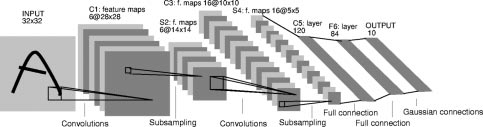
\includegraphics[width=\textwidth]{lecunCNN}
 \caption{Arsitektur dari LeNet-5 \cite{lecun1998gradient}}
   \captionsetup{font={footnotesize}}
  \caption*{Sumber: \citet{lecun1998gradient}, halaman 6}
 \label{fig:lecun}   
\end{figure}

Convolutional Neural Networks menggabungkan tiga buah ide arsitektur yaitu local receptive fields (local connection), shared weights dan spatial subsampling \citet{lecun1998gradient}. Shared weights mampu menghilangkan overfitting atau proses training berlebihan dan local connection dapat mengurangi banyaknya parameter dan kompleksitas \citet{hinton2010practical}. Pada Gambar~\ref{fig:lecun}, terdapat arsitektur dari CNN untuk pengenalan karakter pada tulisan tangan yang disebut dengan LeNet-5. Pada arsitektur tersebut terdiri dari tiga jenis layer yaitu layer Convolution, Sub Sampling dan Full Connection (Fully-connected Layer). Pada perkembangannya,\textit{sub sampling} akan menggunakan istilah pooling yaitu merupakan bentuk sampling non-linier. Terdapat beberapa fungsi non linier dimana yang paling sering digunakan adalah fungsi Max Pooling.

Pada CNN, masukan berupa gambar diambil pada bagian tertentu dengan metode sliding window. Setiap data yang diambil dari proses tersebut dikirimkan pada layer selanjutnya yaitu layer convolution berupa masukan.

\begin{figure}[ht]
 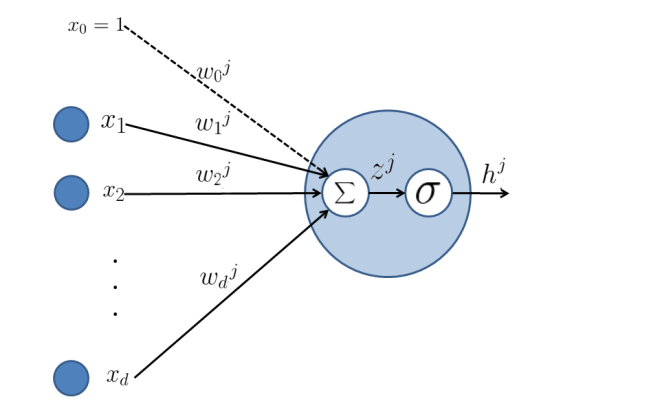
\includegraphics[width=\textwidth]{perceptron}
 \caption{Perceptron dengan Bias dan Input Sebanyak d}
 \label{fig:perceptron}   
\end{figure}

Convolution layer merupakan layer inti dari arsitektur CNN. Terlihat pada Gambar~\ref{fig:perceptron} yang menggambarkan proses mulai dari masukan hingga keluaran pada Layer ini. Layer ini terdiri dari dua tahap yaitu penjumlahan antar pembebanan ($\Sigma$) dan operasi non linier ($\sigma$). Masukan biasa di tuliskan dengan $x_{i}$ dimana i merupakan nomor masukan yang dimulai dari 1 hingga d. Variabel $x_{0}$ merupakan bias yang biasanya diisikan dengan angka 1. Notasi $w_{i}^{(j)}$ merupakan pembebanan (weight) pada input i pada layer j. Nilai dari penjumlahan antar pembebenan didapatkan dari persamaan berikut ini

\begin{equation}
Z^{j} = (\sum_{i=1}^{d} w_{i}^{(j)} * x_{i}) + w_{0}^{(j)}x_{0}
\end{equation}

Setelah proses penjumlahan tersebut, nilai $Z^(j)$ akan dimasukan pada fungsi non linier dengan persamaan sebagai berikut
\begin{equation}
h^{(j)} = \sigma Z^{(j)}
\end{equation}

Selanjutnya adalah layer pooling. Pada Max Pooling yaitu layer yang mampu membagi gambar masukan ke dalam satu set persegi panjang lalu pada masing masing persegi penajang tersebut akan diberikan keluaran berupa nilai maksimumnya. Biasanya, layer ini dimasukan setelah layer convolution untuk mengurangi banyaknya parameter dan komputasi pada jaringan serta kontrol terhadap overfitting. Seperti terlihat pada Gambar~\ref{fig:maxpooling}, dengan adanya Max Pooling membuat layer selanjutnya hanya perlu memproses data empat kali lebih kecil.

\begin{figure}[ht]
  \centering
 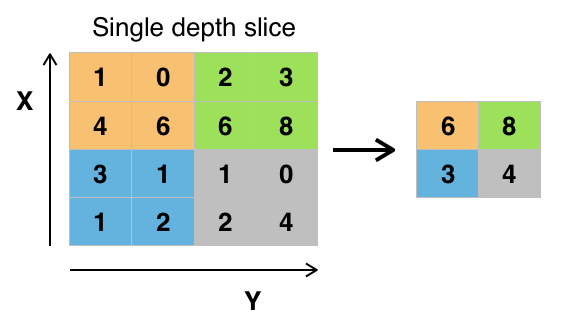
\includegraphics[width=0.7\textwidth]{maxpooling}
 \caption{Max Pooling dengan Filter 2x2}
   \captionsetup{font={footnotesize}}
  \caption*{Sumber:  Aphex34 - Own work, CC BY-SA 4.0, https://commons.wikimedia.org/w/index.php?curid=45673581 (diakses tanggal 25 Juli 2016)}
 \label{fig:maxpooling}   
\end{figure}

Pada layer terakhir biasanya diberikan fully connected layer setelah beberapa layer convolution dan pooling. Banyaknya layer convolution dan pooling yang dibutuhkan tidak bisa ditentukan hingga proses eksperimen menunjukan nilai yang optimal. Setiap neuron di layer fully connected saling terhubung bahkan juga dengan layer sebelumnya. Dengan adanya hubungan tersebut, akan dilakukan prediksi hingga didapatkan keputusan sesuai dengan program yang dirancang. Untuk dapat mengetahui perbandingan antara nilai prediksi dan nilai aktual maka digunakan sebuah persamaan cost function. Jika diasumsikan banyaknya training samples adalah N, maka cost function dari CNN sebagai berikut
\begin{equation}
 E = \frac{1}{2} \sum_{n=1}^{N} (t^{n} - y^{n})^{2}
\end{equation}

Sebelumnya telah disebutkan bahwa pada arsitektur CNN, terdapat tiga layer utama yaitu Convolutional Layer, Pooling Layer dan Fully-Connected Layer. \citet{krizhevsky2012imagenet} mampu menghasilkan peningkatan kecepatan training yang signifikan dengan menambahkan layer Rectified Linier Units (ReLU) pada non-saturating activation function atau pada non linier. Persamaan ReLU dapat dituliskan sebagai persamaan di bawah
\begin{equation}
 f(x) = (1+e^{-x})^{-1}
\end{equation}

Hasil akhir dari keseluruhan proses tersebut menghasilkan keputusan apakah gambar masukan terdapat korban atau tidak. Keputusan tersebut mendasari aksi selanjutnya yang akan dilakukan.

\subsection{Paper Object Detection}
Salah satu pengembangan arsitektur CNN yang cukup fenomenal adalah CNN dengan deteksi berbasis \textit{region}. Penelitian awal dilakukan oleh \citet{girshick2014rich} yang diberi nama R-CNN (R untuk Region, berbeda dengan RNN dengan R adalah Recurrent). Pada perkembangannya, R-CNN dilakukan optimalisasi dalam segi kecepatan dengan berbagai cara seperti SPPnet\cite{he2014spatial}, Fast R-CNN\cite{girshick2015fast} dan yang paling mutakhir saat ini Faster R-CNN\cite{ren2015faster}.

\begin{figure}[ht]
  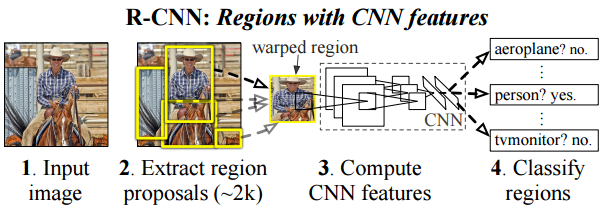
\includegraphics[width=\textwidth]{rcnn}
  \caption{Konsep R-CNN}
     \captionsetup{font={footnotesize}}
  \caption*{Sumber: \citet{girshick2014rich}, halaman 1}
  \label{fig:rcnn}
\end{figure}
Tujuan dari R-CNN adalah menyelesaikan masalah dalam deteksi objek. Pada algoritma R-CNN, gambar yang diberikan akan digambar sebuah kotak (bounding box) pada semua objek yang terdeteksi. Proses terbagi atas dua tahap yaitu region proposal dan klasifikasi. Seperti terlihat pada Gambar~\ref{fig:rcnn}, Gambarmasukan akan dilakukan ekstraksi region proposal dengan menggunakan selective search dan menghasilkan sekitar 2000 region yang berbeda. Pada setiap region akan dilakukan perhitungan dengan CNN menggunakan AlexNet sehingga didapatkan feature dari setiap region. Feature tersebut digunakan sebagai masukan untuk melakukan klasifikasi. 

R-CNN memiliki performa deteksi yang baik namun membutuhkan waktu yang cukup lambat karena menjalankan CNN pada setiap region proposal tanpa melakukan \textit{sharing computation}. SPPnet mampu membuat fixed-length representation tanpa terpengaruh dari ukuran gambar. SPPnet mampu menghitung feature maps dari seluruh gambar hanya dalam satu waktu lalu menggabungkan region untuk membuat representasi dari objek. SPPnet mampu memberikan peningkatan kecepatan testing R-CNN sebanyak 24 hingga 64 kali dan mengurangi waktu yang dibutuhkan sebanyak 3 kali. Metode SPPnet mampu menghitung feature map dengan konvolusi pada seluruh gambar masukan dan menklasifikasi setiap object proposal.

\begin{figure}[ht]
  \centering
  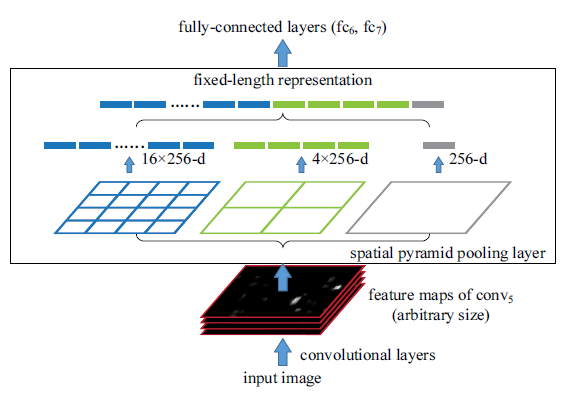
\includegraphics[width=0.75\textwidth]{SPPnet}
  \caption{Konsep SPPnet}
       \captionsetup{font={footnotesize}}
  \caption*{Sumber: \citet{he2014spatial}, halaman 3}
  \label{fig:SPPnet}
\end{figure}

Terlihat pada Gambar~\ref{fig:SPPnet}, berbeda dengan R-CNN yang melakukan konvolusi pada region yang didapat, SPPnet melakukan konvolusi pada gambar masukan lalu dimasukan kedalam Spatial Pyramid Pooling. Feature yang memiliki ukuran yang berbeda-beda akan disesuaikan sehingga didapatkan fixed-length representation. Keluaran dari SPP tersebut dimasukan dalam layer fully connected dan didapatkan loss.

\begin{figure}[ht]
  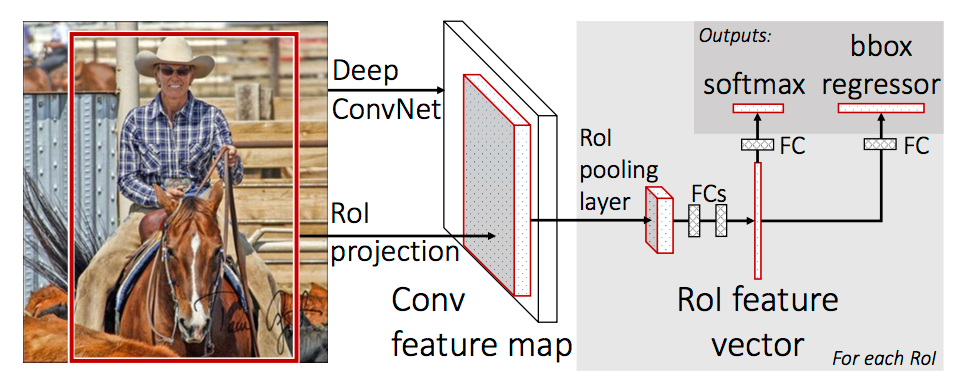
\includegraphics[width=\textwidth]{fast_rcnn}
  \caption{Konsep Fast R-CNN}
       \captionsetup{font={footnotesize}}
  \caption*{Sumber: \citet{girshick2015fast}, halaman 2}
  \label{fig:fast_rcnn}
\end{figure}

Fast R-CNN hadir untuk melakukan peningkatan dalam tiga masalah utama yaitu training membutuhkan beberapa tahapan (CNN lalu SVM / Softmax lalu regresi Bounding Box), komputasi tidak efisien (\textit{expensive}) dan proses yang sangat lama (RCNN membutuhkan 53 detik per gambar). Pada dasarnya Fast R-CNN melakukan \textit{sharing computation} dari layer konvolusi diantara proposal dan menukar urutan proses pembuatan region proposal dengan proses CNN. Model ini secara sederhana terlihat pada Gambar~\ref{fig:fast_rcnn}, dimana dilakukan CNN terlebih dahulu hingga layer ke 5 dan masuk kedalam region proposal (RoI pooling layer). RoI layer secara sederhana merupakan pengembangan dari SPPnet dengan melakukan pooling pada sub-window. Fungsi akhir dilakukan fully connected layer dan didapatkan loss dan bbox regressor.

\begin{figure}[ht]
  \centering
  \begin{subfigure}[b]{0.47\textwidth}
    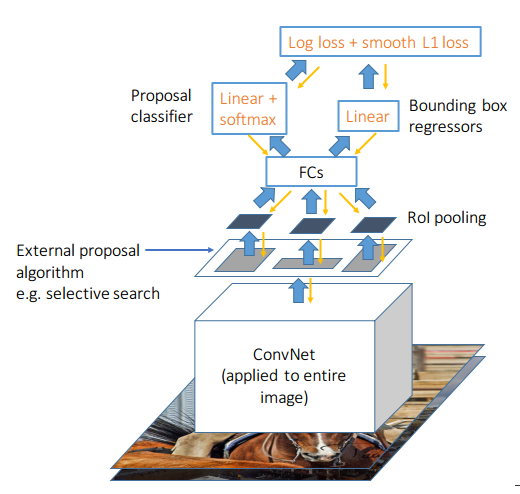
\includegraphics[width=\textwidth]{scheme-rcnn}
    \caption{}
    \label{fig:fast}   
  \end{subfigure}             
  \begin{subfigure}[b]{0.47\textwidth}
    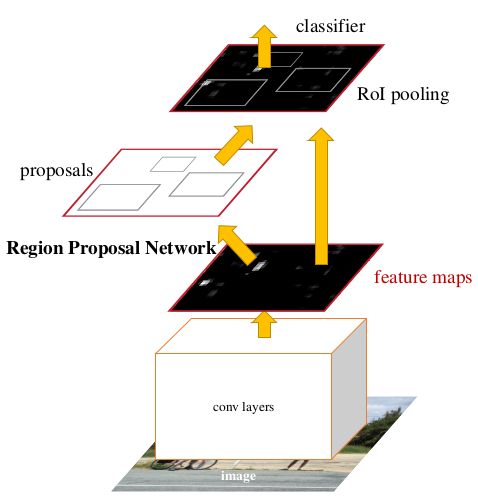
\includegraphics[width=\textwidth]{fasterrcnn_rpn}
    \caption{}
    \label{fig:faster}
  \end{subfigure}
  \caption{Gambaran Sederhana Dari Network (a) Fast R-CNN (b) Faster R-CNN}
       \captionsetup{font={footnotesize}}
  \caption*{Sumber: \citet{ren2015faster}, halaman 3}
  \label{fig:fasterrcnn_rpn}
\end{figure}

Fast R-CNN memiliki kelemahan pada metode object proposal pada region proposal yang menyebabkan terjadinya \textit{bottleneck}. Secara sederhana, Faster R-CNN adalah Fast R-CNN ditambah dengan Region Proposal Network (RPN) yang dapat dilihat perbedaannya di Gambar~\ref{fig:fasterrcnn_rpn}. RPN tersebut dapat berbagi features dari hasil konvolusi gambar penuh sehingga dapat mendapatkan \textit{cost-free} region proposals seperti pada Gambar~\ref{fig:share_features}. RPN tersebut secara simultan memprediksi objek pada setiap posisi.

\begin{figure}[ht]
\centering
 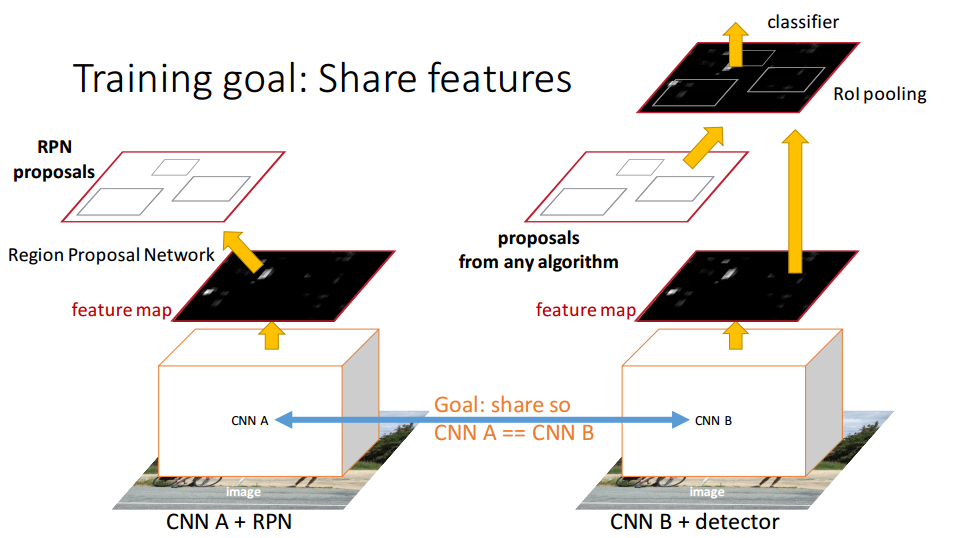
\includegraphics[width=0.8\textwidth]{share_features}
 \caption{Share Feature yang Dilakukan RPN}
      \captionsetup{font={footnotesize}}
  \caption*{Sumber: \citet{girshick2015tutorial}, halaman 37}
 \label{fig:share_features}   
\end{figure}

Faster R-CNN memperkenalkan dua algoritma baru yang dapat dilakukan yaitu Alternating Optimization \cite{ren2015faster} dan Approximate Joint Training. Pada Alternating Optimization, dilakukan empat kali proses training dan dua kali membuat objek proposal. Secara berurutan dapat dilihat proses learning pada Gambar~\ref{fig:alt_opt}. Berbeda dari Alternating Optimization yang terdiri dari beberapa tahap, Approximate Joint Training merangkumnya menjadi satu tahap konvolusi dan RPN untuk dilakukan learning satu kali. Approximate Joint Training memiliki mean Avarage Precision (mAP) sedikit lebih besar namun memiliki perbedaan waktu lebih cepat yang cukup signifikan.

\begin{figure}[ht]
\centering
 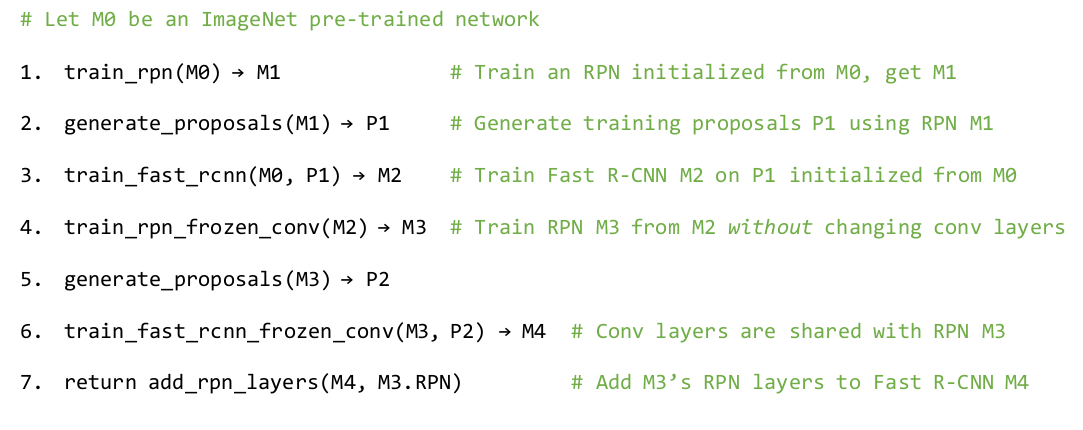
\includegraphics[width=0.8\textwidth]{alt_opt}
 \caption{Faster R-CNN Alternating Optimization}
      \captionsetup{font={footnotesize}}
  \caption*{Sumber: \citet{girshick2015tutorial}, halaman 38}
 \label{fig:alt_opt}   
\end{figure}

Pada bagian konvolusi di Faster R-CNN, dapat dipilih tiga net yang berbeda yaitu VGG16 \cite{simonyan2014very}, VGG CNN M 1024 \cite{chatfield2014return} dan ZFnet \cite{zeiler2014visualizing}. VGG16 memiliki 13 shareable convolutional layers sehinga net ini disebut dengan Very Deep Network. Sedangkan ZFnet hanya menggunakan 5 shareable convolutional layers. VGG CNN M 1024 memiliki layer yang terinspirasi dari ZFnet dengan mengurangi langkah dan memperkecil bidang penerimaan pada layer awal.

\subsection{Deep Learning Library}

Caffe \citet{jia2014caffe} merupakan sebuah Deep Learning Framework yang dibuat oleh Yangqing Jia dan dikembangkan oleh Berkeley Vision and Learning (BVLC), UC Berkeley dan komunitas \textit{open source}. Caffe menklaim memiliki kelebihan pada arsitektur yang mudah, pengembangan yang masif, cepat dalam pemrosesan dan memiliki komunitas yang besar.

Secara anatomi, Caffe terdiri dari Net, Layer dan Blob. Blob merupakan mekanisme penyimpanan data yang merupakan variabel standar N-dimensional array yang digunakan untuk proses transfer data antara CPU dan GPU. Dimensi pada Blob pada umumnya terdiri dari 4-dimensi dengan informasi $N number x K channel x H height x W width$. Number memberikan informasi jumlah batch pada sebuah data sedangkan Channel merupakan fitur yang terdapat pada gambar (misalnya RGB memiliki 3 K).

Layer merupakan bagian dasar pemodelan Deep Learning sebagai dasar bagian penghitungan. Setidaknya terdapat empat kategori utama yang disediakan digunakan untuk membangun pemodelan yang disajikan sebagai berikut. Layer yang paling sering digunakan ditandai dengan huruf tebal.

\begin{itemize}
 \item Vision Layers
 \begin{itemize}
  \item \textbf{Convolution}
  \item \textbf{Pooling}
  \item \textbf{Local Response Normalization (LRN)}
  \item im2col
 \end{itemize}

 \item Loss Layers
 \begin{itemize}
  \item \textbf{Softmax}
  \item Sum-of-squares / Euclidean
  \item Hinge / Margin
  \item Sigmoid Cross-Entropy
  \item Infogain
  \item Accuracy and Top-K
 \end{itemize}
 
 \item Activation / Neuron Layers
  \begin{itemize}
  \item \textbf{Rectified Linear Unit (ReLU)}
  \item Sigmoid
  \item TanH (Hyperbolic Tangent)
  \item Absolute Value
  \item Power
  \item BNLL
 \end{itemize}
 
 \item Data Layers
   \begin{itemize}
  \item \textbf{Database}
  \item In-memory
  \item HDF5 Input
  \item Images
  \item Windows
  \item \textbf{Dummy}
 \end{itemize}
 \item Common Layers
   \begin{itemize}
  \item \textbf{Inner Product (Fully Connected)}
  \item Splitting
  \item Flattening
  \item \textbf{Reshape}
  \item Concatenation
  \item Slicing
  \item Elementwise Operations
  \item Argmax
  \item Softmax
  \item Mean-Variance Normalization
 \end{itemize}
\end{itemize}

Perancangan hubungan antar layer disebut dengan nama Net. Net tertulis pada sebuah format protobuf atau prototxt. Terdapat dua jenis Net yaitu \textit{Backward} dimana setiap variabel akan dapat berubah dan digunakan untuk learning serta \textit{Forward} dimana akan menggunakan hasil training untuk melakukan klasifikasi dari gambar yang didapatkan. Net dapat divisualisasikan sehingga terlihat pada Gambar~\ref{fig:ketlayer} (b) dan cara membacanya disajikan pada (a).

\begin{figure}[ht]
  \centering
  \begin{subfigure}[b]{0.9\textwidth}
     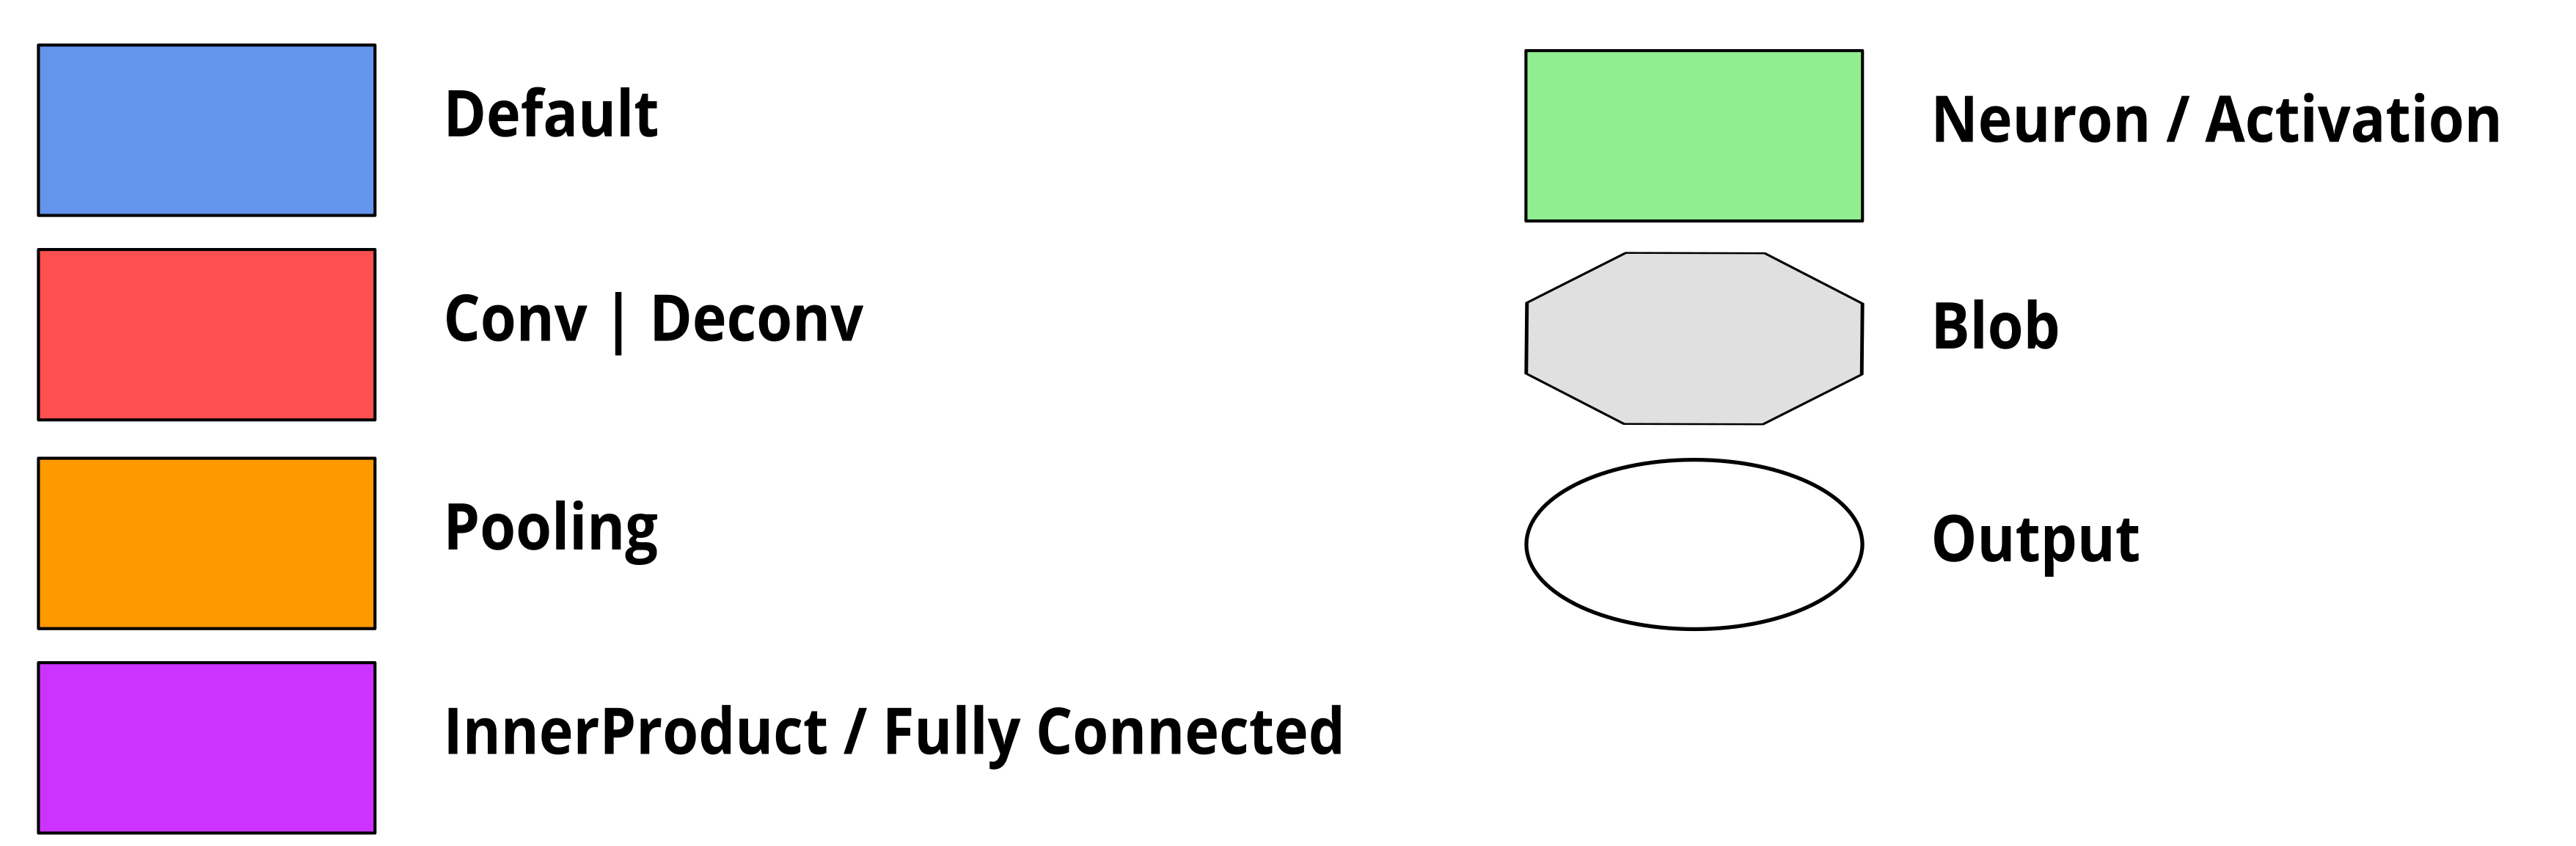
\includegraphics[width=\textwidth]{ketlayer}
     \caption{}
  \end{subfigure}             
  \begin{subfigure}[b]{0.7\textwidth}
    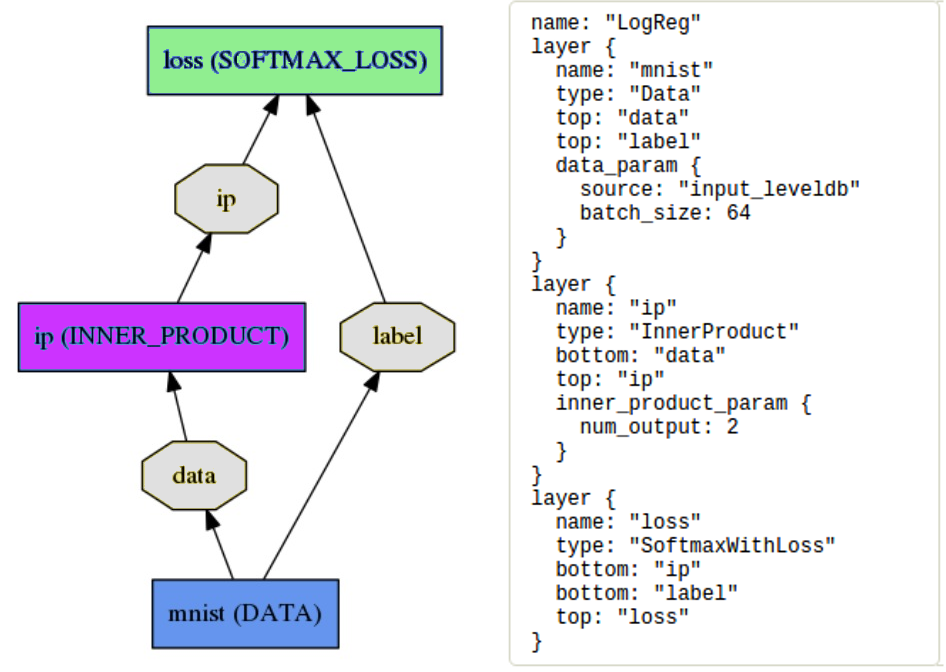
\includegraphics[width=\textwidth]{visualisasi_protobuf}
    \caption{}
  \end{subfigure}
  \caption{(a) Cara Membaca Net (b) Visualisasi dari Net dan Penulisannya pada Protobuf}
  \label{fig:ketlayer}
\end{figure}

Caffe pada dasarnya berjalan menggunakan bahasa C++ serta mendukung antarmuka bahasa Python dan Matlab. Caffe dapat berjalan menggunakan CPU maupun GPU hanya dengan mendefinisikan pada $Caffe::mode()$. Setiap layer didefinisikan pada sebuah format \textit{plaintext protocol buffer schema} (prototxt) dimana ketika selesai melakukan \textit{learning} akan menjadi \textit{binary protocol buffer} dengan ekstensi $.caffemodel$. Caffemodel tersebut akan digunakan pada Net forward untuk dijadikan referensi klasifikasi objek.